\documentclass{article}
\usepackage{amsmath}
\usepackage[utf8]{inputenc}
\usepackage[T1]{fontenc}
\usepackage[ngerman]{babel}
\usepackage[shortlabels]{enumitem}
\usepackage{amsfonts}
\usepackage[left=3cm,right=2cm,top=2.5cm,bottom=2cm]{geometry}
\usepackage{xcolor}
\usepackage{algorithm}
\usepackage{amssymb}
\usepackage[noend]{algpseudocode}
\usepackage{tikz}
\usepackage{mathtools}

\title{Algorithmen und Datenstrukturen: Übung 4}
\author{Tanja Zast, Alexander Waldenmaier}

\begin{document}
    \maketitle

    \subsection*{Aufgabe 4.1}
    \begin{enumerate}
        \item[a)] Wenn mit Wahrscheinlichkeit $p'=\frac{2}{3}$ zwei Marsianer am selben Tag Geburtstag haben, dann beträgt die Wahrscheinlichkeit für völlig unterschiedliche Geburtstage $p = \frac{1}{3}$. Mit $m=687$ ergibt die Formel aus dem Skript dann für die gesuchte Anzahl $n$ an Marsianern: 
        \begin{align*}
            \prod_{i=1}^{n-1} \frac{m-1}{m} = p &\approx e^{-\frac{\left(n-\frac{1}{2}\right)^2}{2m}} \\
            \ln p &\approx -\frac{\left(n-\frac{1}{2}\right)^2}{2m} \\
            2m \ln p &\approx -\left(n-\frac{1}{2}\right)^2 \\
            \sqrt{- 2m \ln p} &\approx n - \frac{1}{2} \\
            n &\approx \sqrt{- 2m \ln p} + \frac{1}{2} \\
            n &\approx \sqrt{- 2 \cdot 687 \ln \frac{1}{3}} + \frac{1}{2} \approx 39,3522 \\
            \Rightarrow n &= 40
        \end{align*}
        Ab 40 Marsianern beträgt die Wahrscheinlichkeit für mindestens eine Dopplung der Geburtstage mehr als $\frac{2}{3}$. 
        \item[b)] Die Wahrscheinlichkeit, dass bei $n$ Einträgen in einer $m$ großen Hashtabelle eine Kollision auftritt, beträgt:
        \begin{align*}
            p = 1 - \prod_{i=1}^{n-1} \frac{m-1}{m} &\approx 1- e^{-\frac{\left(n-\frac{1}{2}\right)^2}{2m}}
        \end{align*}
        Mit der Bedingung $p> \frac{2}{3}$ und unter Verwendung der Approximation folgt:
        \begin{align*}
            \frac{2}{3} &\lesssim 1- e^{-\frac{\left(n-\frac{1}{2}\right)^2}{2m}} \\
            \frac{1}{3} &\gtrsim e^{-\frac{\left(n-\frac{1}{2}\right)^2}{2m}} \\
            \ln \frac{1}{3} &\gtrsim -\frac{\left(n-\frac{1}{2}\right)^2}{2m} \\
            2m \ln \frac{1}{3} &\gtrsim -\left(n-\frac{1}{2}\right)^2 \\
            \sqrt{- 2m \ln \frac{1}{3}} &\lesssim n - \frac{1}{2} \\
            n &\gtrsim \sqrt{- 2m \ln \frac{1}{3}} + \frac{1}{2}
        \end{align*}
    \end{enumerate}

    \subsection*{Aufgabe 4.2}
    Gegeben: $S = \{92, 19, 83, 37, 16, 57, 61\}, m=11$
    \begin{enumerate}
        \item[a)] \hfill \\
        \begin{minipage}[t]{0.3 \textwidth}
            \begin{tikzpicture}[baseline=(current bounding box.north)]
                \coordinate (0);
                \foreach \t/\n[count=\i from 0,evaluate=\i as\j using int(\i+1)] in {
                    / \slash ,
                    / \slash ,
                    57 \slash / ,
                    / \slash ,
                    92 $\rightarrow$ 37 \slash / ,
                    16 \slash / ,
                    83 $\rightarrow$ 61 \slash / ,
                    / \slash ,
                    19 \slash / ,
                    / \slash ,
                    / \slash
                }
                \node at(\i.south)[anchor=north,draw,minimum height=2em,minimum width=2.5em,outer sep=0pt](\j){\n}
                    node at(\j.west)[align=right,left]{\i} 
                    node at(\j.east)[align=left,right,xshift=-.7em]{$\rightarrow$ \t};
            \end{tikzpicture} 
        \end{minipage} 
        \begin{minipage}[t]{0.4\textwidth}
            Es entstehen zwei Kollisionen: 92 kollidiert mit 57 am Index 4, 83 kollidiert mit 61 am Index 6.
        \end{minipage}

        \item[b)]
        \begin{minipage}[t]{0.3 \textwidth}
            \begin{tikzpicture}[baseline=(current bounding box.north)]
                \coordinate (0);
                \foreach \t/\n[count=\i from 0,evaluate=\i as\j using int(\i+1)] in {
                    / \slash ,
                    / \slash ,
                    57 \slash / ,
                    / \slash ,
                    92 \slash / ,
                    37 \slash / ,
                    83 \slash / ,
                    16 \slash / ,
                    19 \slash / ,
                    61 \slash / ,
                    / \slash
                }
                \node at(\i.south)[anchor=north,draw,minimum height=2em,minimum width=2.5em,outer sep=0pt](\j){\n}
                    node at(\j.west)[align=right,left]{\i} 
                    node at(\j.east)[align=left,right,xshift=-.7em]{$\rightarrow$ \t};
            \end{tikzpicture} 
        \end{minipage} 
        \begin{minipage}[t]{0.4\textwidth}
            \begin{tabular}{l|ccccccc}
                $s$ & 92 & 19 & 83 & 37 & 16 & 57 & 61 \\ \hline
                $i$ & 0 & 0 & 0 & 1 & 2 & 0 & 3
            \end{tabular} \\\\
            Es entstehen insgesamt 6 Kollisionen. 
        \end{minipage}
        
        \item[c)]
        \begin{minipage}[t]{0.3 \textwidth}
            \begin{tikzpicture}[baseline=(current bounding box.north)]
                \coordinate (0);
                \foreach \t/\n[count=\i from 0,evaluate=\i as\j using int(\i+1)] in {
                    / \slash,
                    37 \slash / ,
                    57 \slash / ,
                    / \slash ,
                    92 \slash / ,
                    16 \slash / ,
                    83 \slash / ,
                    61 \slash / ,
                    19 \slash / ,
                    / \slash ,
                    / \slash
                }
                \node at(\i.south)[anchor=north,draw,minimum height=2em,minimum width=2.5em,outer sep=0pt](\j){\n}
                    node at(\j.west)[align=right,left]{\i} 
                    node at(\j.east)[align=left,right,xshift=-.7em]{$\rightarrow$ \t};
            \end{tikzpicture} 
        \end{minipage} 
        \begin{minipage}[t]{0.4\textwidth}
            \begin{align*}
                h(37, 1) &= (h_1(37) + 1\cdot h_2(37)) \mod{11} \\
                &= (4 + (1+ ((37 -1 ) \mod{(11-1)}))) \mod{11} \\
                &= (4 + (1 + 36 \mod{10})) \mod{11} \\
                &= (4 + 4) \mod{11} \\
                &= 8 \\\\
                h(37, 2) &= (h_1(37) + 2\cdot h_2(37)) \mod{11} \\
                &= (4 + 2 \cdot 4) \mod{11} \\
                &= 1 \\\\
                h(61, 1) &= (h_1(61) + 1\cdot h_2(61)) \mod{11} \\
                &= (6 + (1+ ((61 - 1) \mod{(11-1)}))) \mod{11} \\
                &= (4 + (1 + 60 \mod{10})) \mod{11} \\
                &= (4 + 1) \mod{11} \\
                &= 5 \\\\
                h(61, 2) &= (h_1(61) + 2\cdot h_2(61)) \mod{11} \\
                &= (4 + 2\cdot 1) \mod{11} \\
                &= 6 \\\\
                h(61, 3) &= (h_1(61) + 2\cdot h_2(61)) \mod{11} \\
                &= (4 + 3\cdot 1) \mod{11} \\
                &= 7
            \end{align*} 
            \begin{tabular}{l|ccccccc}
                $s$ & 92 & 19 & 83 & 37 & 16 & 57 & 61 \\ \hline
                $i$ & 0 & 0 & 0 & 2 & 0 & 0 & 3
            \end{tabular} \\\\
            Es entstehen insgesamt 5 Kollisionen. 
        \end{minipage}
    \end{enumerate}


    \subsection*{Aufgabe 4.3}
    Aussage:
    \begin{align*}
        A: \forall h(s_i) \exists s_1, s_2 \in S \subset U \:|\: n = |S|, |U| > m(n-1) : h(s_1) = h(s_2)
    \end{align*}
    Gegenaussage:
    \begin{align*}
        \bar{A}: \forall h(s_i) \forall s_1, s_2 \in S \subset U \:|\: n = |S|, |U| > m(n-1) : h(s_1) \neq h(s_2)
    \end{align*}
    Die Gegenaussage gilt es nun zu widerlegen. \\
    Damit alle Schlüssel des Universums einen eigenen Platz in der Hashtabelle bekommen können (sonst würden zwangsläufig Kollisionen auftreten),
    muss gelten: 
    \begin{align*}
        m &\ge |U| \\
        \stackrel{\bar{A}}{\Rightarrow} m &\ge |U| \stackrel{!}{>} m(n-1) \\
        m &\ngeq m(n-1), \text{mit } n \ge 2
    \end{align*}
    Die Gegenaussage wurde widerlegt, womit $A$ gilt. 


    \subsection*{Aufgabe 4.4}
    Wir nehmen an, dass zwei unterschiedliche Werte $x_1, x_2$ durch die $k$ Hash-Funktionen auf die selben Indizes abgebildet werden. Ist $x_1$ bereits gespeichert, dann werden beim Abspeichern von $x_2$ keine Bits verändert. Wird nun beispielswiese $x_1$ gelöscht, so würde eine Abfrage (bloomCheck) von $x_2$ \textit{false} ergeben, da alle zugehörigen Bits bei der Löschung von $x_1$ auf \textit{false} gesetzt wurden. Das widerspricht dem Anspruch des BloomFilters, keine False Negatives herauszugeben. 


    \subsection*{Aufgabe 4.5}
    Qualitativ lässt sich sagen: Je mehr Hash-Funktionen, desto geringer sollte die Wahrscheinlichkeit für false positives werden, da die Anzahl an Bits, die identisch sein müssen, zunimmt. Andererseits werden mit mehr Hash-Funktionen auch mehr Bits befüllt, der Belegungsgrad wird höher, wodurch irgendwann wieder mehr false positives auftreten. Dies zeigt sich an der Formel aus dem Skript:

    \begin{align*}
        P(\text{false positive}) &= (1-p)^k \\
        &\approx (1 - \underbrace{e^{-\frac{nk}{m}}}_{\mathclap{p=P(A[i]=\mathrm{FALSE})}})^k 
    \end{align*}
    Die minimale Kollisionswahrscheinlichkeit liegt bei $k=7$ vor. Im Folgenden sind die Werte für alle zulässigen $k$ und $n=100, m=1000$ aufgetragen und grafisch dargestellt:\\\\
    \begin{tabular}{l|ccccccccccc}
        $k$ & 2 & 3 & 4 & 5 & 6 & 7 & 8 & 9 & 10 & 11 & 12 \\ \hline
        $P$ [\%] & 3.2859 & 1.7411 & 1.1813 & 0.9431 & 0.8436 & 0.8194 & 0.8455 & 0.9127 & 1.0186 & 1.1650 & 1.3561
    \end{tabular}
    \begin{figure}[h]
        \centering
        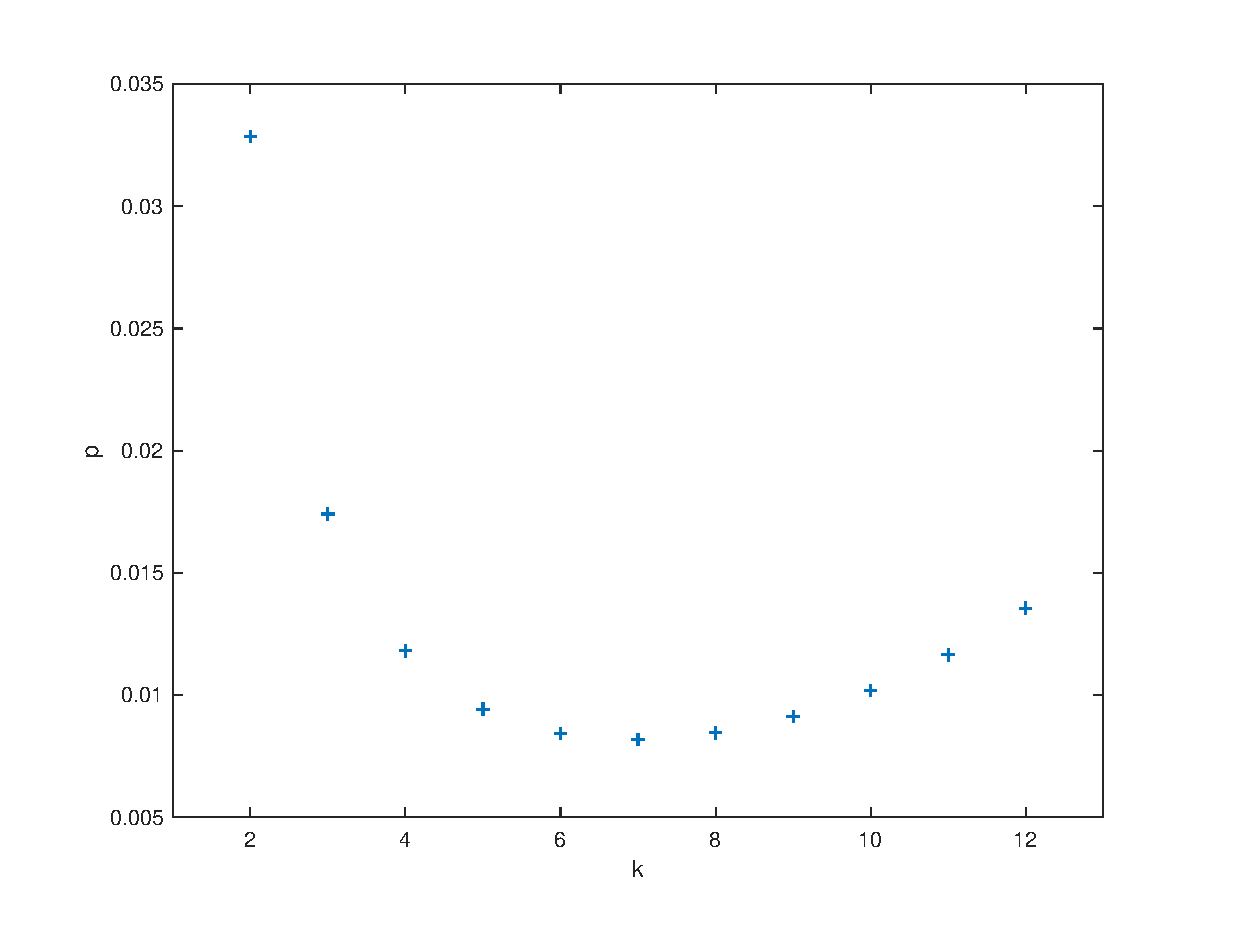
\includegraphics[width=0.7\textwidth]{plot_4_4.eps}
        \caption{Wahrscheinlichkeit $p$ für false positives bei $k$ Hash-Funktionen ($n=100, m=1000$)}
    \end{figure}
    

    \subsection*{Aufgabe 4.6}
    Abgabe in DOMjudge. Teamname: "test"

\end{document}